\documentclass[11pt, titlepage]{article}
\usepackage{amsmath,amsthm,amssymb}
\usepackage{hyperref, pgf, tikz}
\usepackage{fancyhdr}
\usetikzlibrary{arrows}
\usepackage[margin=1.25in]{geometry}
\usepackage{graphicx}
\pagestyle{fancy}
\usepackage{array}
%\usepackage{wrapfig}

\lhead{Lab \#04}
\rhead{\thepage}
\cfoot{}

\title{\Huge{Torques, Equilibrium, and Center of Gravity} \\ \ \\ \huge Lab \#04}
\author{\Large{Alon Levin} \\ \emph{Lab Partner: Sophia Zheng}}
\date{\today}
\begin{document}

\maketitle

\begin{center}
\LARGE Torques, Equilibrium, and Center of Gravity
\end{center}

\section*{Objective}
The objective of this lab is to explain mechanical equilibrium \& how it is applied to rigid bodies, to distinguish between center of mass \& center of gravity, and to describe how a laboratory beam balance measures mass.

\section*{Introduction}
In \textbf{mechanical equilibrium}, the vector sums of the forces $\vec{F}$ and torques $\vec{\tau}$ acting on a body are zero; furthermore, if it is in \textbf{static equilibrium}, the object's linear and angular velocities are zero as well. As mechanical equilibrium has two conditions, each condition is a specific type of equilibrium as well.

\textbf{Translational equilibrium} refers to the condition that $\Sigma \vec{F} = 0$; this ensures that the object is either not moving linearly (i.e., that it remains at a particular location) or that it is moving with uniform linear velocity (i.e., that it is not accelerating, by Newton's First Law of Motion).

\textbf{Rotational equilibrium} refers to the condition that $\Sigma \vec{\tau} = 0$; this ensures that the object is either not rotating, or that it rotates with a uniform angular velocity. For static equilibrium to occur, both translational and rotational equilibriums have to be static --- in other words, the object should be neither moving nor rotating.

Torque $\tau$ is the result of an application of a force $F$ acting perpendicularly on an object a distance $r$ (called the moment arm or lever arm) from the axis of rotation. The full formula for torque is $\vec{\tau} = \vec{r} \times \vec{F}$; its magnitude is thus $\tau = rF\sin\theta$. Convention tells us that the positive direction for torque is counterclockwise. For rotational equilibrium to occur, the sum of the counterclockwise torques has to be equal to the sum of the counterclockwise torques.

The \textbf{center of gravity} of a rigid body is the point at which the sum of the gravitational torques about an axis through this point is zero. The \textbf{center of mass} of a rigid body, however, is the point at which the distribution of mass is centered around. As long as $g$ is constant, the two points are the same.

\textbf{Linear mass density} $\mu$ is the mass per unit length. It is found by dividing the total mass $m$ by the total length $L$ ($\mu = \frac{m}{L}$), with units of grams/centimeter or kilograms/meter.

\section*{Procedure}
After determining the masses of the meterstick \& clamps and length of the meterstick, the meterstick should be set up in such a way so that it can rotate about an axis but is fixed in place so that it is in translational equilibrium. Masses can be attached to clamps that slide onto the meterstick and thus allow us to move the masses in such a way as to find static equilibrium. For a diagram, see Fig. \ref{fig:1}.

For the first section, the axis of rotation should be at the meterstick's center of gravity so as to make sure that torque due to gravity is zero, and thus allowing us to focus solely on the masses. We test the three cases, two of which we have to find the location of an additional known mass to create rotational equilibrium, and the third in which we use the method of moments to compare an unknown mass with a known mass by noting the distances at which they create rotational equilibrium.

For the second section, the apparatus is fixed at a point other than its center of gravity; we must now account for the mass of portions of the meterstick when doing our torque calculations. In the first case, we have to find the distance at which the meterstick's torque on one side balances out the sum of the torques due to an object and the second portion of the meterstick. In the second case, we used an uneven distribution of mass (due to positioning) to observe how the position of the center of gravity of the meterstick moves.

\begin{figure}[!ht]
\centering
%\vspace*{1.5cm}
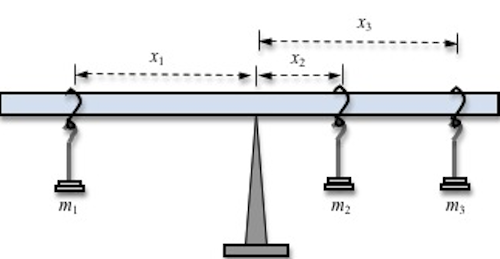
\includegraphics[scale=.8, angle=0]{lab04_setup.png}
\caption{Setup used for this experiment \label{fig:1}}
\end{figure}

\pagebreak
\section*{Data}
\noindent Center of Gravity:
$$x_o = 0.51 ~\text{m}$$
Mass of meterstick:
$$m_m = 0.0631 ~\text{kg}$$
Average mass of one clamp:
$$m_c = 0.01663 ~\text{kg}$$
\begin{center}
\begin{figure}[!ht]
\begin{tabular}
{|m{4em}|m{20em}|m{14em}|}
\hline
Case & Masses (kg) & Coordinate (m)\\
\hline
Case 1 & $m_1 = 0.11663, m_2 = 0.21663$ & $x_1 = 0.15, x_2 = 0.691$ \\
\hline
Case 2a & $m_1 = 0.11663, m_2 = 0.21663, m_3 = 0.06663$ & $x_1 = 0.3, x_2 = 0.7, x_3 = 0.12$ \\
\hline
Case 2b & $m_1 = 0.11663, m_2 = 0.21663, m_3 = 0.06663$ & $x_1 = 0.2, x_2 = 0.6, x_3 = 0.777$ \\
\hline
Case 3 & $m_{1m} = 0.3331, m_2 = 0.21663$ & $x_1 = 0.2, x_2 = 0.9635$ \\
\hline
\end{tabular}
\caption{Apparatus with Point of Support at Center of Gravity \label{table:1}}
\end{figure}

\begin{figure}[!ht]
\begin{tabular}
{|m{4em}|m{20em}|m{14em}|}
\hline
Case & Masses (kg) & Coordinate (m)\\
\hline
Case 5b & $m_1 = 0.11663, m_2 = 0.0631$ & $x_1 = 0, x_2 = .588, x_o' = 0.176$ \\
\hline
Case 5b & $m_1 = 0.11663, m_2 = 0.051994, m_3 = 0.011106$ & $x_1 = 0, x_2 = .588, x_3 = 0.088, x_o' = 0.176$ \\
\hline
Case 6a & $m_1 = 0.11663, m_2 = 0.11663$ & $x_1 = 0, x_2 = 0.6, x_o' = 0.342$\\
\hline
Case 6b& $m_1 = 0.11663, m_2 = 0.11663$ & $x_1 = 0, x_2 = 0.7, x_o' = 0.3825$\\
\hline
Case 6c& $m_1 = 0.11663, m_2 = 0.11663$ & $x_1 = 0, x_2 = 0.8, x_o' = 0.4215$\\
\hline
Case 6d& $m_1 = 0.11663, m_2 = 0.11663$ & $x_1 = 0, x_2 = 0.9, x_{om}' = 0.4657, x_{op}' = 0.462$ \\
\hline
\end{tabular}
\caption{Apparatus Supported at Different Pivot Points \label{table:2}}
\end{figure}

\begin{figure}[!ht]
\hspace{-.5cm}
\begin{tabular}
{|m{4em}|m{9em}|m{7em}|m{7em}|m{9em}|}
\hline
Case & Moment/Lever Arms (m) & Counterclockwise Torque (N*m) & Clockwise Torque (N*m) & Percent Error (Value)\\
\hline
Case 1 & $r_1 = 0.351, r_2 = 0.19$ & 0.4012 & 0.4034 & 0.55\% (Torque)\\
\hline
Case 2a & $r_1 = 0.201, r_2 = 0.199, r_3 = 0.381$ & 0.4180 & 0.4132 & 1.15\% (Torque)\\
\hline
Case 2b & $r_1 = 0.301, r_2 = 0.099, r_{3m} = 0.276, r_{3c} = .281 $ &  &  & 1.81\% ($r_3$)\\ 
\hline
Case 3 & $r_1 = 0.301, r_2 = 0.4625$ &  &  & $m_{1c} = 0.3329; 0.07\%$\\
\hline
\hline
\hline
Case 5a & $r_1 = 0.176, r_2 = 0.412$ & 0.2014  & 0.2550 & 23.5\% (Torque) \\
\hline
Case 5b & $r_1 = 0.176, r_2 = 0.412, r_3 = 0.088$ & 0.2110 & 0.2101 & 0.43\% (Torque) \\
\hline
Case 6a & $r_1 = 0.342, r_2 = 0.258$ &  &  &  \\ 
\hline
Case 6b & $r_1 = 0.3825, r_2 = 0.3175$ &  &  &  \\
\hline
Case 6c & $r_1 = 0.4215, r_2 = 0.3785$ &  &  &  \\
\hline
Case 6d & $r_1 = 0.462, r_2 = 0.438$ & 0.5286 & 0.5011 & 5.34\% (Torque), 0.79\% ($x_o'$) \\
\hline
\end{tabular}
\caption{Calculated Results \label{table:3}}
\end{figure}
\end{center}

\pagebreak
\section*{Discussion}
\subsection*{Sample Calculations}
$$\mu = \frac{m_{m}}{L} = \frac{0.0631}{1} = 0.0631 ~kg/m$$
\noindent Calculations for Case 1
$$\tau_{cc} = m_1r_1g = (0.11663)(0.351)(9.81) = 0.4012 ~N/m$$
$$\tau_{cw} = m_1r_1g = (0.21663)(0.190)(9.81) = 0.4034 ~N/m$$
$$\text{Diff.} = \frac{|0.4012-0.4034|}{\frac{0.4012+0.4034}{2}} \ast 100\% = 0.55\%$$

\pagebreak
\subsection*{Analysis}
The reason that Case 5a stands out in terms of error is due to the fact that the calculations were flawed to begin with. In calculating the torque, we were instructed to assume that the entire weight of the meterstick is applied to the clockwise side and none of it is applied to the counterclockwise side. We then used proper calculations in Case 5b, with the proper parts of the meterstick being applied to their respective sides, and thus found an answer with a significantly smaller percent error.

Otherwise, our percent error was considerably low, staying below 5\% for all but one of the cases (Case 6d). There are three possible causes of error, and none of them would have a major effect on the results: (a) our assumption that the linear density of the meterstick was constant throughout, although this is not necessarily the case; (b) our simplification of the rigid body masses into point masses for calculation purposes; and (c) minute errors in gathering measurements.

\subsection*{Questions}
\begin{enumerate}
\item In our setup, the meterstick was clamped to the support beam in such a way that it was allowed to rotate, but it was supported so as to be in translational equilibrium. The clamp and support beam provided the normal force to counteract the weight of the system, thus providing for the condition $\Sigma \vec{F} = 0$.
\end{enumerate}

\section*{Conclusion}
Case 1 had a counterclockwise torque of 0.4012 N*m to the clockwise torque of 0.4034 N*m for a percent error of 0.55\%. Case 2a had a counterclockwise torque of 0.4180 N*m to the clockwise torque of 0.4132 N*m for a percent error of 1.15\%. Case 2b had an experimentally-measured moment arm $r_{3m} = 0.276$ m to the calculated 0.281 m, for a percent error of 1.81\%. Case 3 had a calculated mass, $m_{1c} = 0.3329$ kg compared to the real mass of 0.3331 kg, for a percent error of 0.07\%.

Case 5a had a counterclockwise torque approximation of 0.2014 N*m, and a clockwise torque approximation of 0.2550 N*m for a 23.5\% difference. Case 5b has a 0.2110 N*m counterclockwise torque approximation, and a 0.2101 N*m clockwise torque approximation for a 0.43\% difference.

Case 6d found $x_o'$ experimentally to be 0.4657 m, as compared to our prediction of 0.462 m, thus giving us a percent difference of 0.79\% and a percent difference between measured torques of 5.34\%.
\end{document}